\section{Testowanie}\label{sec:testowanie}
\subsection{Sieć neuronowa}\label{subsec:testowanie_siec_neuronowa}
Ważnym elementem każdego modelu uczenia maszynowego jest sprawdzenie, jak model radzi sobie z danymi, których nie widział podczas uczenia.
W tym celu wykorzystuje się zbiór testowy zawierający dane, które nie były użyte do trenowania modelu.
Wyniki klasyfikacji na zbiorze testowym są miarą tego, jak dobrze model radzi sobie z nowymi danymi - jak bardzo model jest w stanie generalizować swoją wiedzę.
\begin{table}[H]
    \centering
    \caption{Dokładność i F-miara dla zbioru testowego po 40 epokach}
    \resizebox{0.6\textwidth}{!}{%
        \begin{tabular}{@{}|l|l|l|l|@{}}
            \toprule
                       & Niezbalansowane & Oversampling & Undersampling \\ \midrule
            dokładność & 91\%            & 92\%          & 90\%           \\ \midrule
            F-miara    & 0,91            & 0,92          & 0,90           \\ \bottomrule
        \end{tabular}%
    }
    \label{tab:acc_f_measure_nn}
\end{table}
Powyższa tabela \ref{tab:acc_f_measure_nn} przedstawia wyniki dokładności i F-miary dla zbioru testowego. Widać wyraźnie, 
że wyniki są bardzo zbliżone do siebie różniąc się o maksymalnie 2 punkty procentowe.
F-miara również jest praktycznie taka sama dla wszystkich trzech zbiorów, a co najważniejsze, ich wartość oscyluje w okolicach 90\%. 
Świadczy to o tym, że model radzi sobie dobrze z nowymi danymi oraz
nie ma problemu z rozpoznawaniem klas mniejszościowych.
\subsection{K - NN}\label{subsec:testowanie_knn}
\begin{table}[H]
    \centering
    \caption{Dokładność i F-miara dla zbioru testowego dla k = 3}
    \resizebox{0.6\textwidth}{!}{%
        \begin{tabular}{@{}|l|l|l|l|@{}}
            \toprule
                       & Niezbalansowane & Oversampling & Undersampling \\ \midrule
            dokładność & 94,41\%         & 95,29\%       & 93,38\%        \\ \midrule
            F-miara    & 0,9443          & 0,9508        & 0,9339         \\ \bottomrule
        \end{tabular}%
    }
    \label{tab:acc_f_measure_knn}
\end{table}
W przypadku algorytmu k - NN, wyniki są jeszcze lepsze niż w przypadku sieci neuronowej. Dokładność i F-miara są wyższe o około 3 punkty procentowe,
zaznaczając przy tym zerowy czas uczenia. Można też przedstawić wyniki klasyfikacji w postaci macierzy pomyłek. 
Macierz pomyłek przedstawia liczbę poprawnie i niepoprawnie zaklasyfikowanych obrazów dla każdej klasy.
\begin{figure}[H]
    \centering
    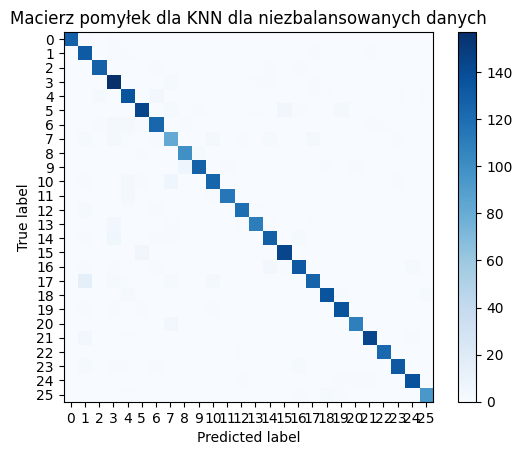
\includegraphics[width=0.5\textwidth]{img/confusion_not_balanced.png}
    \caption{Niezbalansowany zbiór testowy}
    \label{fig:confusion_matrix_knn_unbalanced}
\end{figure}
\begin{figure}[H]
    \begin{subfigure}{0.5\textwidth}
        \centering
        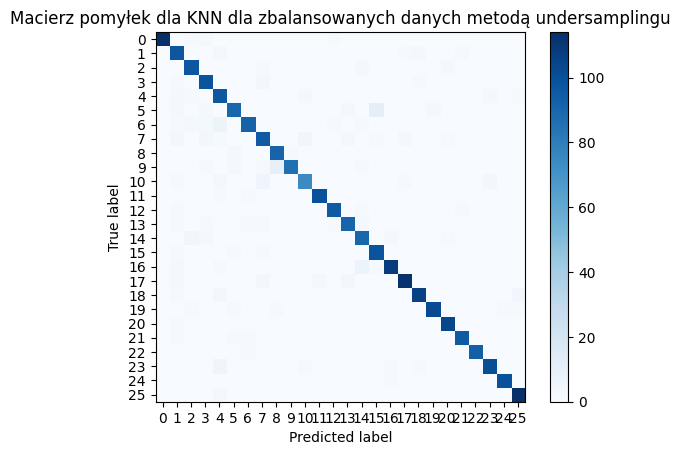
\includegraphics[width=\textwidth]{img/confusion_under.png}
        \caption{Undersampled zbiór testowy}
        \label{fig:confusion_matrix_knn_under}
    \end{subfigure}
    \begin{subfigure}{0.49\textwidth}
        \centering
        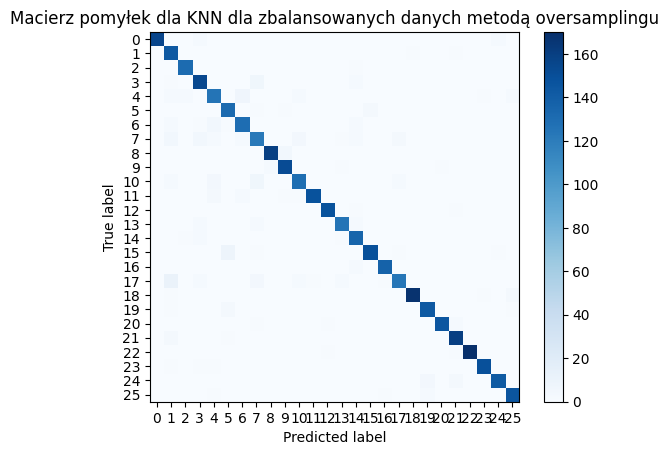
\includegraphics[width=\textwidth]{img/confusion_over.png}
        \caption{Oversampled zbiór testowy}
        \label{fig:confusion_matrix_knn_over}
    \end{subfigure}
\end{figure}
Ze względu na bardzo wysoką dokładność modelu KNN oraz bardzo niską liczbę błędów, macierz pomyłek jest bardzo podobna dla wszystkich trzech przypadków.
Widoczne są bardzo niewyraźne plamy poza przekątną głównej macierzy, co oznacza, że model dobrze radzi sobie z klasyfikacją.
